\documentclass{article}
\usepackage[utf8]{inputenc}
%%%%%%%%%%%%%%%%%%%%%%%%%%%%%%%%%%%%%%%%%%%%%%%%%%%%%%%%%%%%%%%%%%%%%%%%%%%%%%%%%%%%%%%%%%%%%%%%%%%%%%%%%%%%%%%%%%%%%%%%%%%
\usepackage[scientific-notation=true]{siunitx} % Provides the \SI{}{} and \si{} command for typesetting SI units
\usepackage{graphicx} % Required for the inclusion of images
\graphicspath{{images/}}
\usepackage{natbib} % Required to change bibliography style to APA
\usepackage{amsmath} % Required for some math elements 
\usepackage[spanish,activeacute]{babel}
\usepackage{float}
\usepackage[table]{xcolor}
\usepackage[table]{xcolor}
\usepackage{anysize}
\usepackage{caption}
\usepackage{subcaption}
\usepackage{pdfpages}%insertar pdf
\marginsize{1in}{1in}{1in}{1in} 
\usepackage{enumerate}
\usepackage[utf8]{inputenc}
\usepackage{wrapfig}
\usepackage{multirow, array}
\usepackage{graphicx}
\usepackage{flushend}
\usepackage[utf8]{inputenc}
%%%%%%%%%%%%%%%%%%%%%%%%%%%%%%%%%%%%%%%%%%%%%%%%%%%%%%%%%%%%%%%%%%%%%%%%%%%%%%%%%%%%%%%%%%%%%%%%%%%%%%%%%%%%%%%%%%%%%%%%%%%%%%
\newcommand{\HRule}{\rule{\linewidth}{0.5mm}}
\setlength\parindent{0pt} % Removes all indentation from paragraphs

\renewcommand{\labelenumi}{\alph{enumi}.} % Make numbering in the enumerate environment by letter rather than number (e.g. section 6)

\newcolumntype{a}{>{\columncolor[gray]{0.9}}c}
%%%%%%%%%%%%%%%%%%%%%%%%%%%%%%%%%%%%%%%%%%%%%%%%%%%%%%%%%%%%%%%%%%%%%%%%%%%%%%%
\begin{document}
%%%%%%%%%%%%%%%%%%%%%
%PORTADA
%%%%%%%%%%%%%%%%%%%%%
\begin{center}

\includegraphics[width=0.3\textwidth]{Escudo_Unison.png}~\\[1cm]

\textsc{\LARGE Universidad de Sonora}\\[0.1cm]
\textsc{División de Ciencias Exactas y Naturales}\\[0.1cm]
\textsc{Departamento de Física}\\[1.5cm]
%\includegraphics[width=0.3\textwidth]{.png}~\\[1cm]

\HRule \\[0.4cm]
\textsc{Actividad 8: Oscilador de Van Der Pol}\\[0.1cm]
\textsc{Física Computacional I \\[0.1cm]}
\HRule \\[1.5cm]

\textsc{Rolando Abdel Fimbres Grijalva \\[1.0cm]}

\vfill
\textsc{15 de abril de 2018\\[0.1cm]}
\pagenumbering{gobble}
\end{center}
%%%%%%%%%%%%%%%%%%%%%%%%%%%%%%%%%%%%%%%%%%%%
\newpage
\pagenumbering{arabic}
\section{Introducción}
En ésta actividad se estudió el oscilador de Van der Pol, el cual sirve pra comprender una clase de oscilación suave en señales generadas por circuitos particulares. Se pide replicar las imagenes que acompañan al artículo de wikipedia de éste oscilador. Para eso necesitaremos hacer uso de la integración numérica tal y como en las actividades pasadas.\\
\section{Modelo de Van der Pol}
El oscilador de Van der Pol es una clase de oscilacion amortiguada que no es lineal. Ésta puede ser modelada mediante una ecuación diferencial de segundo orden:\\
\begin{center}
${d^{2}x \over dt^{2}}-\mu(1-x^{2}){dx \over dt}+x=0$
\end{center}
El modelo fue propuesto por Balthasar Van der Pol en 1920 mientras estaba empleado por la compañía Philips.\\
\subsection{Historia}
Van der Pol fue un ingeniero y físico. Él encontró oscilaciones estables que decidió llamar de relajación. Hoy en día éstas son comunmente llamadas cíclos límite. Los circuitos empleados en aquella época contaban con tubos de vacío, éstos se hacían funcionar cerca del cíclo límite pues entraban en acoplamiento y entraba en fase con la corriente.\\
\subsection{Forma bidimensional}
Aplicándo el teorema de Liénard se pueden encontrar dos formas, aplicando dos transformaciones. Una de ellas es: $y=x-x^{3}/3-\dot{x}/\mu$, $y=x-x^{3}/3-\dot{x}/\mu$, obteniendo así las ecuaciones:\\
\begin{center}
$\dot{x}=\mu(x-\frac{1}{3}x^{3}-y)$\\
$\dot{y}=\frac{1}{\mu}x$\\
\end{center}
La forma se basa en la transformación $y=\dot{x}$, llevando a la ecuación:\\
\begin{center}
$\dot{x}=y$\\
$\dot{y}=\mu(1-x^{2})y-x$\\
\end{center}
\section{Soluciones del modelo}
Para poder analizar el comportamiento del oscilador es necesario utilizar un código bastante parecido al de lass actividades anteriores ya que el oscilador se modela con ecuaciones diferenciales que pueden integrarse numéricamente. A continuación se mostrarán las gráficas de posición contra tiempo, fase y cíclo límite así como el código utilizado para llegar a ella.\\
Primero se comienza con la definición de los parámetros:\\
\begin{center}[H]
	\centering
    \includegraphics[width=\linewidth]{dp.png}
\end{center}
Después necesitamos ingresar todas las condiciones iniciales para replicar en el diagrama de flujo de campo en wikipedia. En éste caso las condiciones son los definidos por $x$ y $v$ en el código:\\
\begin{center}[H]
	\centering
    \includegraphics[width=\linewidth]{ci0.png}
\end{center}
\begin{center}[H]
	\centering
    \includegraphics[width=\linewidth]{ci1.png}
\end{center}
\begin{center}[H]
	\centering
    \includegraphics[width=\linewidth]{ci2.png}
\end{center}
\begin{center}[H]
	\centering
    \includegraphics[width=\linewidth]{ci3.png}
\end{center}
\begin{center}[H]
	\centering
    \includegraphics[width=\linewidth]{ci4.png}
\end{center}
Ahora se introducirá el código que genera el diagrama de campo.\\
\begin{center}[H]
	\centering
    \includegraphics[width=\linewidth]{f.png}
\end{center}
\begin{center}[H]
	\centering
    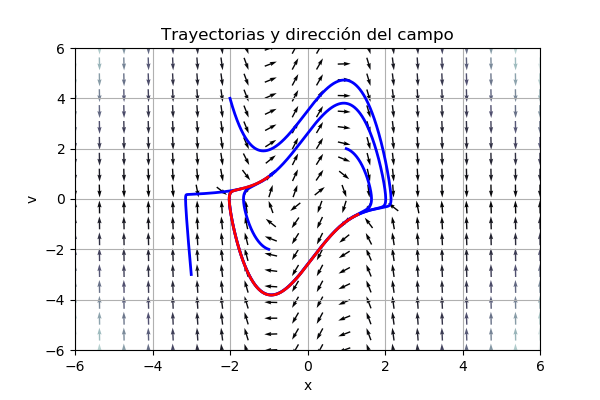
\includegraphics[width=\linewidth]{FasesCondiciones.png}
\end{center}
Después necesitamos el código para mostrar el desplazamiento con respecto al tiempo. El primero son fuerza externa y el segundo con fuerza externa. En el caso del primero:\\
\begin{center}[H]
	\centering
    \includegraphics[width=\linewidth]{d1.png}
\end{center}
Obteniendo:\\
\begin{center}[H]
	\centering
    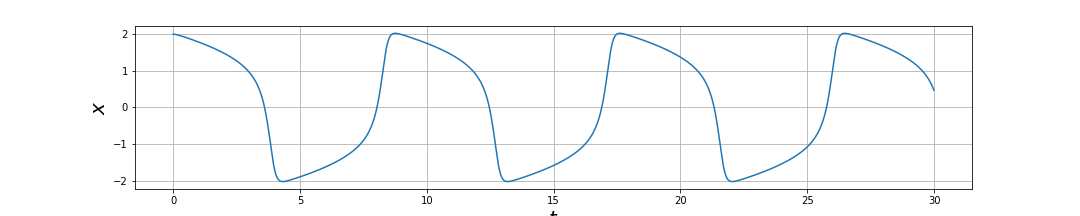
\includegraphics[width=\linewidth]{TerceraFig.png}
\end{center}
En el segundo caso:\\
\begin{center}[H]
	\centering
    \includegraphics[width=\linewidth]{d2.png}
\end{center}
Obteniendo:\\
\begin{center}[H]
	\centering
    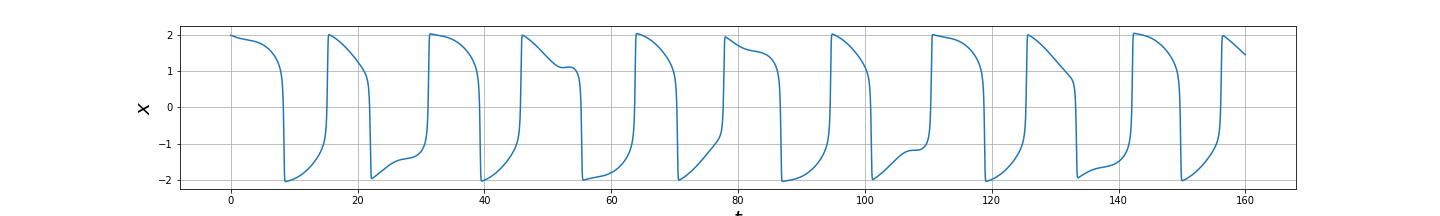
\includegraphics[width=\linewidth]{CuartaFig.png}
\end{center}
También necesitabamos ver el comportamiento cuando $\mu$ varía desde 0.01 hasta 4. 
\begin{center}[H]
	\centering
    \includegraphics[width=\linewidth]{04_1.png}
\end{center}
\begin{center}[H]
	\centering
    \includegraphics[width=\linewidth]{04_2.png}
\end{center}
\begin{center}[H]
	\centering
    \includegraphics[width=\linewidth]{04_3.png}
\end{center}
Obteniendo:\\
\begin{center}[H]
	\centering
    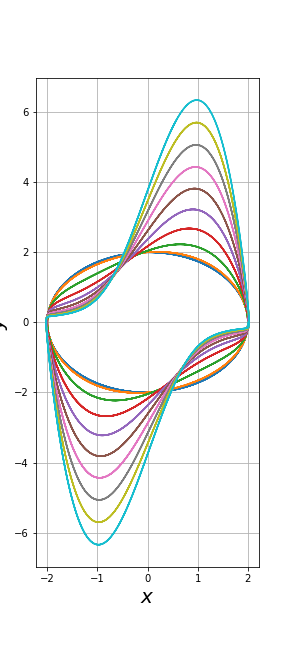
\includegraphics[width=\linewidth]{SegundaFig.png}
\end{center}
\section{Resultados}
Al concluir con la programación y mirar detalladamente los diagramas generados podemos ver que en el primer caso se conto con varias condiciones iniciales. Aun así miramos que siguen el patrón del cíclo límite. Además de como el campo direccional favorece a la trayectoria.\\
En el caso de las graficas de desplazamiento vemos como aun existe una periodicidad notable en la oscilación.\\
Finalmente se observa cómo afecta una fuerza externa a la oscilación aunque se vea muy ligera. Y al cambiarse los coeficientes como se notan picos.\\
\section{Conclusiones}
El tema fué bastante interesante pues se introdujo un nuevo fenómeno que puede ser resuelto con las mismas herramientas numéricas utilizadas con anterioridad. Debo decir que me costó bastante trabajo a comparacion de las prácticas anteriores pues tuve que recurrir a la ayuda de compañeros. Despejadas mis dudas me di cuenta que es muy importante definir los parametros y en mi caso mantener separadas los archivos de datos ya que cometía el error de asignarles un mismo nombre cosa que complicaba todo.\\
\section{Bibliografía}
Matplotlib: Lotka-Volterra tutorial -SciPy Cookbook doc. 2018.\\
Van der Pol oscillator. 2018., www.scholarpedia.org\\
\section{Apéndice}
1.Éste ejercicio pareciera similar al desarrollo en las catividades 6 y 7. ¿Qué aprendiste nuevo?\\
A como hacer el campo direccional, ne pareció que fue lo más relevante.\\
2.¿Qué fue lo que más te llamó la atención del oscilador de Van der Pol?\\
El hecho de que los circuitos con los que Van der Pol trabajaba funcionaban cerca del cíclo límite.\\
3.Has escuchado ya hablar de caos. ¿Por qué sería importante estudiar éste oscilador?\\
Si. Lo considero importante porque me parece que los fenómenos más complejos y que mayor impacto hacia el humano tienen son sistemas caóticos.\\
4.¿Qué mejorarías de ésta actividad?\\
No sería una mejora, tal vez lo que yo haría sería separarla en dos actividades distintas. Me pareció muy extensa.\\
5.¿Algún comentario adicional antes de dejar de trabajar en Jupyter con Python?\\
Que me parece un lenguaje más sencillo y práctico que FORTRAN. Y jupyter fue nuevo para mi. Me parece muy bien y que solo necesitas acceso a internet si no cuenta tu equipo con la aplicación necesaria.\\
6.Cerramos la parte de trabajo con Python ¿qué te ha parecido?\\
Muy bien, práctico, fácil de aprender y me agrada que cuente con una gran cantidad de bibliotecas para realizar una gran variedad de trabajos. Me parece muy útil como herramienta de análisis de datos lo que la vuelve excelente en la física y muchas otras áreas.\\
\end{document}
